\documentclass[crop,tikz,10pt]{standalone}

\usepackage{xcolor}

\definecolor{background}{HTML}{F0F4F5}
\definecolor{border}{HTML}{D3E0E3}

\definecolor{blue}{HTML}{1395ba}
\definecolor{dark_blue}{HTML}{0e708c}

\definecolor{pink}{HTML}{f8216e}
\definecolor{dark_pink}{HTML}{b3174e}

\definecolor{yellow}{HTML}{f8ca00}
\definecolor{orange}{HTML}{ff8a39}

\definecolor{green}{HTML}{4fa400}
\definecolor{dark_green}{HTML}{306400}


\usepackage{tikz}
\usetikzlibrary{
    arrows,
    backgrounds,
    positioning,
}

\begin{document}

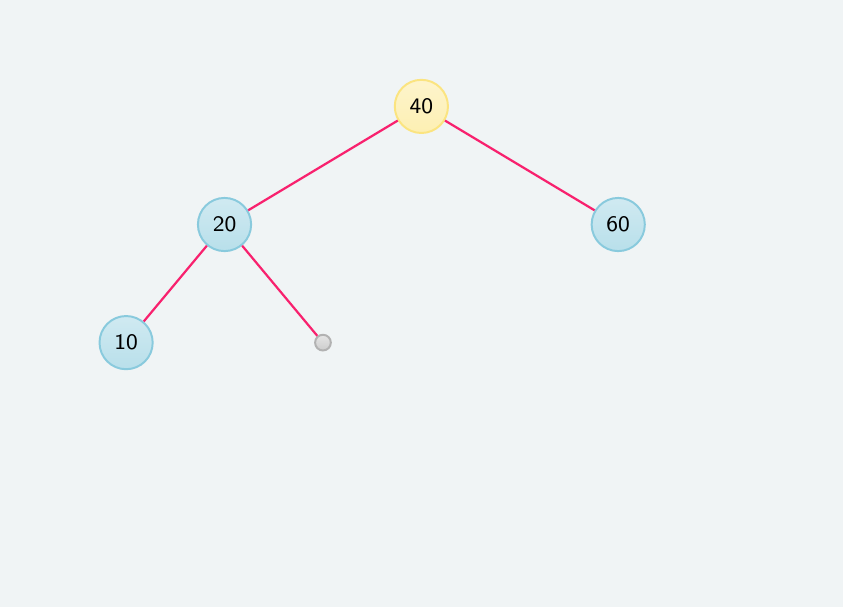
\begin{tikzpicture}[%
    scale=1.0,
    node distance=0.5cm,
    every node/.style={minimum size=0, inner sep=0},
    on grid,
    background rectangle/.style={draw=border!80!black,fill=background},
    show background rectangle,
    inner frame sep=0.5cm,
    level/.style={
        sibling distance = 5cm/#1,
        level distance = 1.5cm
    },
    every node/.style={
        font=\sffamily\footnotesize,
        circle,
        minimum size=0.6cm,
        line width=0.025cm,
        draw=blue!50,
        top color=blue!20,
        bottom color=blue!30,
    },
    root/.style={
        draw=yellow!50,
        top color=yellow!20,
        bottom color=yellow!30,
    },
    null/.style={
        minimum size=0.2cm,
        inner sep=0,
        draw=black!30,
        top color=black!10,
        bottom color=black!20,
    },
    edge from parent/.style={
        draw,
        pink,
        thick
    }
]

\clip (0, 0) rectangle (10.0, 7.0);

\node [root] at (5, 6) {40}
    child {
        node {20} 
        child { 
            node {10}     
        }
        child { 
            node [null] {}    
        }
    }
    child {
        node {60} 
    }
    
;
 
\end{tikzpicture}
\end{document}